\section{Query-based Federated Learning}
\label{sec:query}
\subsection{Overview}
Let us continue by establish a sustainable open FL platform based on a query-based cooperation framework.
An overview of this platform is presented in Fig.~\ref{fig:query}, the desin philosophy behind this framework is to break the coupling between FL server and clients.
In the query-based FL systems, all traditional FL roles and components are maintained on an open model repository called Model Community. The Model Community privdes a one-stop ML models redistribution and reuse service, including model indexing, automatic batch model reuse, license management, privacy control and so on.
In addition to large-scale pretrained models like BERT~\cite{devlin2018bert}, BLOOM~\cite{scao2022bloom} with great generalization abilities, we also encourage individuals to upload their task-specific models trained on limited domain data to boost the knowledge mining within models~\cite{you2021workshop}.
The derivatives of knowledge mining can learn representations from multiple domains, resulting in more promising performance that can be evaluated by platform users.
Furthermore, the contributors can open models under applicable licenses, granting them distribution control and legal protection of their intellectual property (IP).
In summary, the properties of query-based FL are:
(1) \textbf{Model Agnostic}, as there are no restrictions on the types and architectures of the models uploaded by users;
(2) \textbf{Contactless}, as coomunication channels need not be maintained; 
(3) \textbf{Community-powered}, whereby sharing models enrichs the entire community.

Actually, we aim to advocate a novel SaaS~\cite{brereton1999future} ML platform with automatic model reuse integrated, which has potential to leverage the transportability of models to address previously unexplored ML problems.
Due to the high computational demands of deep learning, current ML platforms primarily concentrate on computing, for example, MaaS, MLaaS, FLaaS provide ML models deployment and development services to handle user-specified tasks. (Section~\ref{sec:aas}).
On the other hand, there are several ML platforms provide open model search and download services. 
So, can we leverage leverage off-the-shelf open model platforms to build a query-based FL system?
Unfortunately, these platforms are designed solely for sharing and are no suitable for more advanced functionalities such as model ensemble~\cite{jacobs1991adaptive} and knowledge distillation~\cite{hinton2015distilling}, we will explain the reasons in the following section.

% Model Mining

\begin{figure}[t]
  \centering
  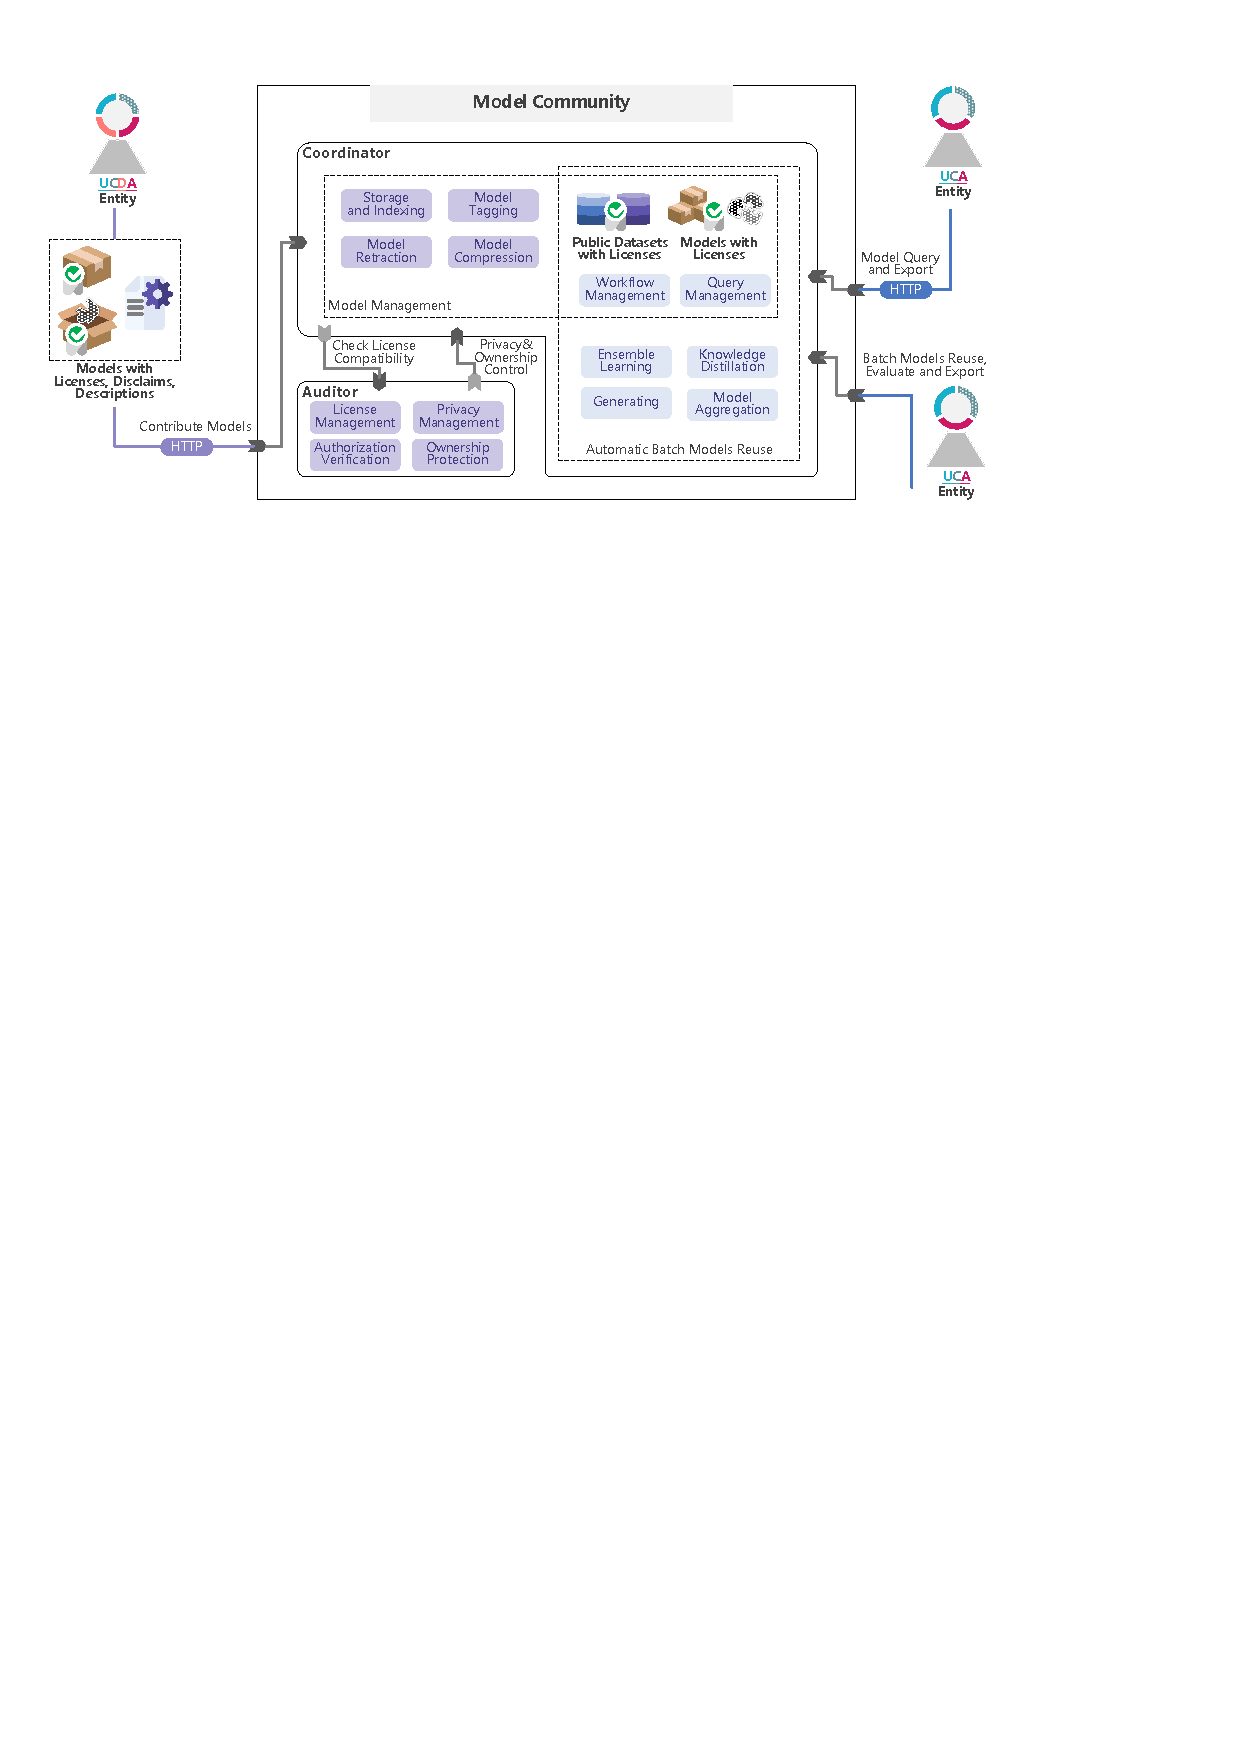
\includegraphics[width=\linewidth]{fig/query_frame.pdf}
  \caption{An overview of query-based FL systems. (U: model User, C: Coordinator, D: Data owner, A: Auditor)}
  \Description{}
  \label{fig:query}
\end{figure}

\subsection{How to Query for Models}
To establish a query-based FL platform, the first thing that comes to mind is how to query for models.
Unlike traditional ML model sharing repositories that mainly query for a specific model by name, it requires an efficiency approach to export a batch of target models that ready for ensemble or distillation.
We summaried the filter conditions of existing DNNs sharing repositories in Table.~\ref{table:repository}.
The prevailing method for querying models involves searching for the desired model by its name, datasets used, associated tasks.
To illustrate, one might search for the model name GPT~\cite{radford2019language}, models trained on the MNIST dataset~\cite{lecun2010mnist}, or models capable of performing image segmentation tasks.
However, this model retrieval method requires the users have a strong priori knowledge in data science, thus raising the barrier for knowledge mining within models.
For example, there is no effective way to acquire a batch of image classfication models that contains the knowledge of \textit{lesser panda} for further distillation.
A compromise solution is to manually search the schema of each dataset one-by-one and subsequently search for models trained on those datasets.

Additionally, as shown in Table.~\ref{table:repository}, most DNNs repositories are simply list the description of input/output (e.g., NVIDIA NGC, OpenVINO) or even just present the source codes (e.g., Tensorflow Hub, Pytorch Hub),
This lack of unified convention for model input/ouput poses a challenge for query-based FL.
Besides, most of DNNs repositories do not enable querying models by licenses, resulting in the cumbersome task of individually handling model licenses and ensuring compatibility among different licenses.
Hence, it is imperative to reconsider the design of DNN repositories to enable quick identification of readily reusable models for model knowledge mining. We further suggest following filter conditions for query-based FL.

\begin{table}[t]
  \caption{Filter conditions and characteristics of DNNs repositories. \checkmark : Supported, \ding{55} : Unsupported, \textbf{!} : Information provided but unsearchable, listed in descending order by number of models.}
  \label{table:repository}
  \footnotesize
  \begin{tabular}{|l|c|c|c|c|c|c|c|c|}
  \hline
  & \multicolumn{1}{l|}{DS Name} & \multicolumn{1}{l|}{Model Architecture} & \multicolumn{1}{l|}{Modality/Task} & \multicolumn{1}{l|}{Tag} & \multicolumn{1}{l|}{License} & \multicolumn{1}{l|}{Input-Output} & \multicolumn{1}{l|}{Batch Export} & \multicolumn{1}{l|}{\# of Models}\\ \hline
  Hugging Face\tablefootnote{https://huggingface.co}
  & \checkmark & \checkmark & \checkmark & \checkmark & \checkmark & \textbf{!} & \ding{55} & 133,641 \\ \hline
  Model Zoo\tablefootnote{https://modelzoo.co/} & \checkmark & \checkmark & \checkmark & \checkmark & \ding{55} & \ding{55} & \ding{55} & 3,426 \\ \hline
  Tensorflow Hub\tablefootnote{https://tfhub.dev/}& \checkmark & \checkmark & \checkmark & \checkmark & \textbf{!} & \textbf{!} & \ding{55} & 1,356 \\ \hline
  NVIDIA NGC\tablefootnote{https://catalog.ngc.nvidia.com/models} & \textbf{!} & \checkmark & \checkmark & \checkmark & \textbf{!} & \textbf{!} & \ding{55} & 527 \\ \hline
  OpenVINO\tablefootnote{https://docs.openvino.ai/latest/model\_zoo.html} & \textbf{!} & \checkmark & \checkmark & \ding{55} & \textbf{!} & \textbf{!} & \checkmark & 278 \\ \hline
  Pytorch Hub\tablefootnote{https://pytorch.org/hub/} & \textbf{!} & \checkmark & \ding{55} & \ding{55} & \ding{55} & \textbf{!} & \ding{55} & 49 \\ \hline
  \end{tabular}
\end{table}

\subsubsection{Data Description} % 数据的domain和统计特征,数据的正确性,如何打标签,
Similar with the data heterogeous challenges in FL~\cite{li2021federated}. The local datasets of contributors have varing quality and contain intractable biases, imbalances and noisies that can be attributed to the natural characteristics of demographic or improper data collection mechanisms~\cite{dayan2021federated}.
Besides, label errors pervasive even in open datasets~\cite{northcutt2021pervasive}. 
So, in addition to searching for domain-specific datasets based on their data descriptions, we are also seeking such descriptions for the purpose of future traceability and debugging.
The data description can consist of statistical analysis results or the visualization diagrams that used to profile the data distribution~\cite{li2020multi} and complementary provenance information.

\subsubsection{Workflow and History}
The process of building an ML model is iterative, involving repeated hyperparameter tuning and architecture exploration, resulting in abundant workflow and historical trajectory data.
This information includes pipelines, model structures, hyperparameter values for pre-training and fine-tuning, test metrics, and results. 
These data can be useful in filtering models that meet specific requirements, such as those with data standardization in preprocessing or evaluated using mean average precision (mAP).
Instead of manually saving and uploading the logs and configuration files, a more efficient method is to leverage ML workflow management tools~\cite{vartak2016modeldb}, such as MLflow~\footnote{https://mlflow.org} and Neptune~\footnote{https://neptune.ai}, to automatically track and store the ML workflow during model building process. 
Additionally, to ensure that the computational consumption of models is within budget, the Deep Learning Profiler~\footnote{https://docs.nvidia.com/deeplearning/frameworks/dlprof-user-guide/index.html} can be leveraged to generate a report that shows the FLOPS and bandwidth requirements.

\subsubsection{Software Dependency}
ML models are software that depend on underlying ML libraries, so it is important to declare the dependencies of the model to analyze software compatibility between batches of models. 
For instance, resource-constrained devices may need to trim down the list of software-dependent libraries to meet limited storage space requirements~\cite{david2021tensorflow}.
In some cases, contributed models may rely on other models as dependencies. 
For example, Fast R-CNN~\cite{girshick2015fast} uses VGG16~\cite{simonyan2014very} as its backbone. 
It is crucial to release this information for further model license compatibility analysis.

The aforementioned filter conditions provide comprehensive coverage of the ML modeling process. 
However, there are additional requirements depending on the reuse mechanisms of the model retrieval side. 
For example, FedAvg~\cite{mcmahan2017communication} aggregates the local models weights element-wise, which requires full access to the models. 
In contrast, MoE with a gating network~\cite{jacobs1991adaptive} only ensembles a batch of model outputs, so the individual models can remain blackboxes in this scenario.
So, in the context of software licenses or model licenses, the batch models reused by FedAvg should be released as source code, while those reused by MoE can be released as binary object code (static linking).
The above distinction is crucial for ensuring that model reuse results meet the legal framework, and this has been overlooked in traditional FL.
We will expand on this topic in the following section.

\subsection{How to Reuse Batch of Models}
Once we have acquired a certain number of models that can contribute to the new target task, the next step is to reuse the knowledge of these pre-trained models, i.e., transfer their knowledge from source domain to the target domain~\cite{pan2009survey}.
However, before deciding on how to reuse the model, it is important to ensure that the necessary legal rights and permissions have been obtained. 
This may involve reviewing the terms and conditions of the licenses under which the models were originally released or obtaining permission from the original creators or copyright holders.
Therefore, in this section, we will not focus on the technical details of how to reuse models, which is already covered by many related surveys, such as Transfer Learning~\cite{pan2009survey}, Ensemble Leanring~\cite{zhou2012ensemble}, Domain Adaptation~\cite{wang2018deep}, Knowledge Distillation~\cite{wang2021knowledge}, Deep Generative Models~\cite{cao2022survey} and Model Fusion~\cite{ji2021emerging}.
Furthermore, the specific model reuse technique or techniques used is at the user's discretion, and the query-based FL platform we advocate is not bound or restricted to any particular model reuse algorithm.
Innovatively, we study how to reuse batch of models, from the perspective of \textbf{legal compliance}.
%Therefore, the focus of this section is how to reuse batch of models, from the perspective of legal compliance.

The machine learning community benefits from the openness of ideas and code, and many high-impact ML conferences and journals encourage authors to publish their source code and dataset to research platforms like Papers With Code~\footnote{https://paperswithcode.com} and Code Ocean~\footnote{https://codeocean.com} to increase exposure and facilitate reproducibility.
To restrict the use of ML techniques for unethical purposes (i.e. Deepfakes~\cite{mirsky2021creation}) and protect the IP of creators, models are typically published under a license agreed upon by the licensor.
Here, we summary the licenses, granted rights, restrictions and enforcements for ML models posted on Hugging Face in Table.~\ref{tab:licenses}.

\subsubsection{Model Licensing Forms}
ML models are licensed in three main forms: as software (e.g. Apache, MIT, GPL), as a model (e.g. OpenRAIL), and as content/database (e.g. CC-BY, PDDL).
The reason for the mixed use of licenses is the ambiguity in the dependency relationship between the code, model, and data.
ML models can be released with reproducable code and be considered as a component of software.
So many open software licenses are naturally deferred for licensing of models.
The most popular license is Apache-2.0, which is a permissive open software license that allows the freedom to make derivative works.
However, the model building process also relies on a massive amount of data~\cite{lecun2015deep} that may be licensed under different licenses, which can lead to license conflicts.
A practical example is BERT~\cite{devlin2018bert}, which was published under the Apache-2.0 license but pre-trained on English Wikipedia documents that are licensed under CC BY-SA 3.0.
This changing of license violates the requirement of the CC BY-SA 3.0, which states that any contribution must be distributed under the \textbf{same license} as the original work.

%We don’t claim ownership of the content you create with GPT-2, so it is yours to do with as you please. We only ask that you use GPT-2 responsibly and clearly indicate your content was created using GPT-2.

From the perspective of content and database licensing, some word embedding models, such as GloVe~\cite{pennington2014glove}, compute vector representations of words based on licensed open linguistic resources.
These representations can be regarded as a translation of corpus and fall under the license of the original linguistic resources.
A more complex scenario arises when the model is fine-tuned with other data that has a different license, for example, fine-tune RoBERTa~\cite{liu2019roberta} (MIT license) with SQuAD2~\cite{rajpurkar2016squad} (CC BY 4.0).
The resulting model can be interpreted as both derived works and combined works.

Not only limited to protecting the IP and controlling the diffusion of ideas, but AI companies and researchers are also concerned about licensees using their models for unethical purposes~\cite{jobin2019global, awad2018moral, yuste2017four}, which is not restricted by traditional licenses based on the context of software and content.
We can infer the concerns of the inventors of GPT-2~\cite{radford2019language} about the unethical use of the model from its modified MIT license, which states, \textit{We don't claim ownership of the content you create with GPT-2, so it is yours to do with as you please. We only ask that you use GPT-2 responsibly and clearly indicate your content was created using GPT-2.} 
However, such a statement lacks legal enforcement, and users may avoid accountability by convincing themselves that despite their efforts to minimize harm, they could not predict the AI artifact they generated would be used for harmful purposes.
Besides, the original licensing frameworks (e.g. MIT, CC BY) for software and content are not well suited to the data-driven ML. 
Many ML operations, such as training, fine-tuning, inference, and distillation, are not explicitly defined in traditional software and content licenses, leaving a potential legal loophole for licensees.

To address the unique challenges and considerations surrounding the use and distribution of ML models, several specific licenses for ML models have been proposed. 
The CreativeML OpenRAIL-M license, proposed by Responsible AI~\cite{contractor2022behavioral}, is the most popular model-specific license on Hugging Face and enables legally enforceable responsible use.
By accepting this license, licensees must adhere to the use-based restrictions stated by the licensor, and these restrictions must also apply to derivative works.
With a multitude of different model licenses available, it becomes a challenging and tedious task to reuse them in bulk. 
It is therefore imperative to establish guidelines for selecting a license for models that are ready for query-based FL.

\begin{table}[t]
  \centering
  \scriptsize
  \caption{Licenses for ML models available on Hugging Face with a focus on their rights, restrictions and enforcements, grouped by free software licenses, AI model licenses, free content or database licenses in descending order of number of models (GPL, BSD, LGPL, CC licenses with unspecified versions are excluded, the similar revisions are merged). \checkmark : Permited or Required, \ding{55} : Not Permited or Not Required, \textbf{!} : Not Explicitly Permited, * : Copyleft License}
  \label{tab:licenses}
  \begin{tabular}{r||ccc|ccc|cccc|c|p{3.5cm}}
    \toprule
    Licenses
    & \multicolumn{1}{P{90}{2.0cm}}{Modify / Merge} &
      \multicolumn{1}{P{90}{2.0cm}}{Redistribution} &
      \multicolumn{1}{P{90}{2.0cm}}{Sublicensing} & 
      \multicolumn{1}{P{90}{2.0cm}}{Commercial Use} & 
      \multicolumn{1}{P{90}{2.0cm}}{Patent Use} & 
      \multicolumn{1}{P{90}{2.0cm}}{Trademark Use} &
      \multicolumn{1}{P{90}{2.0cm}}{State Changes} &
      \multicolumn{1}{P{90}{2.0cm}}{Disclose Source} &
      \multicolumn{1}{P{90}{2.0cm}}{Responsible-use Restrictions} &
      \multicolumn{1}{P{90}{2.0cm}}{License/Disclaim Preservation} &
      \multicolumn{1}{P{90}{2.0cm}}{\# of Models} &
      \multicolumn{1}{c}{Licensed Materials / Remarks}    \\
    \midrule
    Apache-2.0 & \checkmark & \checkmark & \checkmark & \checkmark & \checkmark & \ding{55} & \checkmark & \ding{55} & \ding{55} & \checkmark & 23,519 & BERT~\cite{devlin2018bert} \\
    MIT &  \checkmark & \checkmark & \checkmark & \checkmark & \textbf{!} & \textbf{!} & \ding{55} & \ding{55} & \ding{55} & \checkmark & 9,605 & GPT-2~\cite{radford2019language} \\
    AFL-3.0 & \checkmark & \checkmark & \checkmark & \checkmark & \checkmark & \ding{55} & \checkmark & \ding{55} & \ding{55} & \checkmark & 1,561 & Italian-Legal-BERT~\cite{licari2022italian} \\
    *GPL-3.0 & \checkmark & \checkmark & \ding{55} & \checkmark & \checkmark & \ding{55} & \checkmark & \checkmark & \ding{55} & \checkmark & 404 & CKIP BERT Chinese \\
    Artistic-2.0 & \checkmark & \checkmark & \checkmark & \checkmark & \checkmark & \ding{55} & \checkmark & \ding{55} & \ding{55} & \checkmark & 331 & Include original source \\
    BSD-3-Clause\&-Clear & \checkmark & \checkmark & \checkmark & \checkmark & \textbf{!} & \textbf{!} & \ding{55} & \ding{55} & \ding{55} & \checkmark & 209 & CodeGen~\cite{nijkamp2022conversational} / A MIT-style license \\
    WTFPL-2.0 & \checkmark & \checkmark & \textbf{!} & \checkmark & \textbf{!} & \textbf{!} & \ding{55} & \ding{55} & \ding{55} & \ding{55} & 131 & A MIT-style permissive license  \\
    *AGPL-3.0 & \checkmark & \checkmark & \ding{55} & \checkmark & \checkmark & \ding{55} & \checkmark & \checkmark & \ding{55} & \checkmark & 96 & Distributed under AGPL only  \\
    Unlicense & \checkmark & \checkmark & \textbf{!} & \checkmark & \textbf{!} & \textbf{!} & \ding{55} & \ding{55} & \ding{55} & \ding{55} & 90 & A MIT-style permissive license  \\
    %GPL & 1 & 2 & 3 & 4 & 5 & 6 & 7 & 8 & 9 & 10 & 63 &  \\
    BSL-1.0 & \checkmark & \checkmark & \checkmark & \checkmark & \textbf{!} & \textbf{!} & \ding{55} & \ding{55} & \ding{55} & \checkmark & 60 & A MIT-style permissive license \\
    %BSD & 1 & 2 & 3 & 4 & 5 & 6 & 7 & 8 & 9 & 10 & 43 &  \\
    *GPL-2.0 & \checkmark & \checkmark & \ding{55} & \checkmark & \textbf{!} & \textbf{!} & \checkmark & \checkmark & \ding{55} & \checkmark & 34 & Not compatible with GPL-3.0  \\
    BSD-2-Clause & \checkmark & \checkmark & \checkmark & \checkmark & \textbf{!} & \textbf{!} & \ding{55} & \ding{55} & \ding{55} & \checkmark & 34 & A MIT-style permissive license  \\
    *LGPL-2.1\&3.0 & \checkmark & \checkmark & \ding{55} & \checkmark & \textbf{!} & \textbf{!} & \checkmark & \checkmark & \ding{55} & \checkmark & 25 & For software libraries  \\
    *OSL-3.0 & \checkmark & \checkmark & \checkmark & \checkmark & \checkmark & \ding{55} & \checkmark & \checkmark & \ding{55} & \checkmark & 22 & Linking is not derivative work \\
    %BSD-3-Clause-Clear & 1 & 2 & 3 & 4 & 5 & 6 & 7 & 8 & 9 & 10 & 14 &  \\
    %LGPL & 1 & 2 & 3 & 4 & 5 & 6 & 7 & 8 & 9 & 10 & 12 &  \\
    ECL-2.0 & \checkmark & \checkmark & \checkmark & \checkmark & \checkmark & \ding{55} & \checkmark & \ding{55} & \ding{55} & \checkmark & 12 & For education communities \\
    *MPL-2.0 & \checkmark & \checkmark & \checkmark & \checkmark & \checkmark & \ding{55} & \checkmark & \checkmark & \ding{55} & \checkmark & 9 & State changes under MPL only  \\
    ISC & \checkmark & \checkmark & \textbf{!} & \checkmark & \textbf{!} & \textbf{!} & \ding{55} & \ding{55} & \ding{55} & \checkmark & 8 & MIT-style license w/o sublicense \\ % Permission to distribute this software for any purpose
    Zlib & \checkmark & \checkmark & \textbf{!} & \checkmark & \textbf{!} & \textbf{!} & \ding{55} & \ding{55} & \ding{55} & \checkmark & 8 & Rename if modified \\
    *Ms-PL & \checkmark & \checkmark & \checkmark & \checkmark & \checkmark & \ding{55} & \ding{55} & \ding{55} & \ding{55} & \checkmark & 7 & Weak copyleft license \\ % Weak copyleft
    *EPL-1.0\&2.0 & \checkmark & \checkmark & \checkmark & \checkmark & \checkmark & \textbf{!} & \ding{55} & \checkmark & \ding{55} & \checkmark & 6 & Can link proprietary license code \\
    NCSA & \checkmark & \checkmark & \checkmark & \checkmark & \textbf{!} & \ding{55} & \ding{55} & \ding{55} & \ding{55} & \checkmark & 4 & Include full text of license \\
    PostgreSQL & \checkmark & \checkmark & \textbf{!} & \checkmark & \textbf{!} & \textbf{!} & \ding{55} & \ding{55} & \ding{55} & \checkmark & 2 & A MIT-style license \\
    OFL-1.1 & \checkmark & \checkmark & \ding{55} & \checkmark & \textbf{!} & \textbf{!} & \ding{55} & \ding{55} & \ding{55} & \checkmark & 2 & For font software \\
    %EPL-1.0 & 1 & 2 & 3 & 4 & 5 & 6 & 7 & 8 & 9 & 10 & 2 &  \\
    *EUPL-1.1 & \checkmark & \checkmark & \checkmark & \checkmark & \checkmark & \ding{55} & \checkmark & \checkmark & \ding{55} & \checkmark & 1 & License of EU covers SaaS \\
    %LGPL-2.1 & 1 & 2 & 3 & 4 & 5 & 6 & 7 & 8 & 9 & 10 & 1 &  \\
    LPPL-1.3c & \checkmark & \checkmark & \checkmark & \checkmark & \textbf{!} & \ding{55} & \checkmark & \checkmark & \ding{55} & \checkmark & 1 & Covering  stewardship transfer \\
    
    \hline
    %\textbf{Model Licenses $\downarrow$} & \multicolumn{12}{l}{} \\
    \hline
    
    CreativeML-OpenRAIL-M & \checkmark & \checkmark & \checkmark & \checkmark & \checkmark & \ding{55} & \checkmark & \ding{55} & \checkmark & \checkmark & 3,590 & Stable Diffusions v1~\cite{rombach2022high} \\
    OpenRAIL &  \multicolumn{10}{l|}{>Responsible AI License template, w/o full text} & 2,393 & ControlNet~\cite{zhang2023adding}  \\
    BigScience-BLOOM-RAIL-1.0 & \checkmark & \checkmark & \checkmark & \checkmark & \checkmark & \ding{55} & \checkmark & \ding{55} & \checkmark & \checkmark & 196 & BLOOM~\cite{scao2022bloom} \\
    BigScience-OpenRAIL-M & \multicolumn{10}{l|}{>Same as BigScience-BLOOM-RAIL-1.0} & 155 & A general version of 1.0 \\
    OpenRAIL++ & \multicolumn{10}{l|}{>Same as CreativeML-OpenRAIL-M} & 72 & Stable Diffusion v2~\cite{rombach2022high} \\
    OPT-175B & \checkmark & \ding{55} & \ding{55} & \ding{55} & \ding{55} & \ding{55} & \ding{55} & \ding{55} & \checkmark & \checkmark & $\approx66$ & OPT LLM~\cite{zhang2022opt} \\
    SEER &  \multicolumn{10}{l|}{>Same as OPT-175B, ban on reverse-engineer} & / & SEER Vision Model~\cite{goyal2022vision} \\
    
    \hline
    \hline

    CC-BY-4.0\&3.0\&2.5\&2.0 & \checkmark & \checkmark & \textbf{!} & \checkmark & \ding{55} & \ding{55} & \checkmark & \ding{55} & \ding{55} & \checkmark & 1,740 & RoBERTa-SQuAD2.0~\cite{rajpurkar2016squad} \\
    *CC-BY-SA-4.0\&3.0 &  \checkmark & \checkmark & \ding{55} & \checkmark & \ding{55} & \ding{55} & \checkmark & \checkmark & \ding{55} & \checkmark & 590 & LEGAL-BERT~\cite{chalkidis2020legal} \\
    *CC-BY-NC-SA-4.0\&3.0 & \checkmark & \checkmark & \ding{55} & \ding{55} & \ding{55} & \ding{55} & \checkmark & \checkmark & \ding{55} & \checkmark & 556 & LayoutLMv3~\cite{huang2022layoutlmv3} \\
    CC-BY-NC-4.0\&3.0\&2.0 & \checkmark & \checkmark & \ding{55} & \ding{55} & \ding{55} & \ding{55} & \checkmark & \ding{55} & \ding{55} & \checkmark & 499 & GALACTICA~\cite{taylor2022galactica} \\
    CC0-1.0 & \checkmark & \checkmark & \textbf{!} & \checkmark & \ding{55} & \ding{55} & \ding{55} & \ding{55} & \ding{55} & \ding{55} & 165 & BlueBERT~\cite{peng2019transfer} \\
    CC-BY-NC-ND-4.0\&3.0 & \checkmark & \ding{55} & \ding{55} & \ding{55} & \ding{55} & \ding{55} & \ding{55} & \ding{55} & \ding{55} & \checkmark & 21 & NonCommercial, NoDerivatives \\
    PDDL & \checkmark & \checkmark & \ding{55} & \checkmark & \ding{55} & \ding{55} & \ding{55} & \ding{55} & \ding{55} & \ding{55} & 16 & Database-specific license \\
    C-UDA & \checkmark & \checkmark & \checkmark & \ding{55} & \textbf{!} & \textbf{!} & \ding{55} & \ding{55} & \checkmark & \checkmark & 13 & Data for computational use only \\
    *LGPL-LR & \checkmark & \checkmark & \ding{55} & \checkmark & \textbf{!} & \textbf{!} & \checkmark & \checkmark & \ding{55} & \checkmark & 12 & LGPL for linguistic resources \\ %如果仅仅发布embedding模型,那么属于“使用语言资源的作品”,如果包含了语言资源或者加密后的资源,那么属于“使用语言资源的衍生物”,包含在此license范围
    *GFDL &  \multicolumn{10}{l|}{>Same as GPL, a free document license} & 12 & txtai-wikipedia \\
    CC-BY-ND-4.0 & \checkmark & \ding{55} & \ding{55} & \checkmark & \ding{55} & \ding{55} & \checkmark & \ding{55} & \ding{55} & \checkmark & 11 & Disallow making derivatives \\
    ODC-By & \checkmark & \checkmark & \ding{55} & \checkmark & \ding{55} & \ding{55} & \ding{55} & \ding{55} & \ding{55} & \checkmark & 7 & Automatic relicensing \\
    %但是只对derivative dataset有定义,对于model来可能不适用
    *ODbL & \checkmark & \checkmark & \ding{55} & \checkmark & \ding{55} & \ding{55} & \checkmark & \checkmark & \ding{55} & \checkmark & 6 & Automatic relicensing \\
    \bottomrule
  \end{tabular}
\end{table}

%The effect of copyleft-style behavioral-use clauses spreads the requirement from the original licensor on his/her wish and trust on the responsible use of the licensed artifact. This is why OpenRAILs require downstream adoption of the use-based restrictions by subsequent re-distribution and derivatives of the AI artifact, as a means to dissuade users of derivatives of the AI artifact from misusing the latter.

%OPT-175B/SEER LICENSE is not a copyleft license, as it does not require derivative works to be licensed under the same license or a compatible one. It is a proprietary license that allows users to use and reproduce the licensed models subject to certain restrictions.

\subsubsection{License Choosing Preferences}
In query-based FL, the model community automatically reuses models contributed by users, which raises unique concerns about licensing of models:
\begin{itemize}
  \item A model license ready for open FL paltforms should allow the \textbf{modification, combination and redistribution} of original works and any derived works; and
  \item \textbf{Sublicensing} right should be granted to lubricate the republication of derived works resulting from knowledge mining; note
  \item Some licenses enforce the source of the derived works to be \textbf{disclosed} and prohibit their \textbf{commercial use}, which hinders model selling~\cite{chen2019towards}; and
  \item Some licenses are \textbf{copyleft} (marked with * in Table.~\ref{tab:licenses}), which means the derivatives must be licensed under the same license or a compatible one, leading to potential license conflicts and proliferation~\cite{gomulkiewicz2009open}; last
  \item All granted rights are preferably \textbf{irrevocable} by the licensors~\cite{reddy2009jacobsen}.
\end{itemize}

Besides, it is important to consider the licensing of two other components when building and reusing models: data and algorithms, which may have entirely different license terms. 
Here, we present several strategies for selecting licenses in query-based FL to minimize conflicts.

\textbf{Preferences for Datasets or Databases}: CC0-1.0, ODC-By > CC BY > C-UDA > LGPL-LR.
% 对于数据:训练:C-UDA 可以sublicense,但是不能商用。CC0 和 CC-BY 可用但是没明确sublicense,ODbL 自动license,但是copyleft,必须开源。对于finetune,除了上述数据外还可LGPL-LP
   
  Our recommended licenses for training datasets and databases for query-based FL are CC0-1.0, ODC-By, and CC BY. CC BY-4.0 is preferred due to the grant of \textit{Sui Generis Database Rights (Art.1c)}. 
  CC0-1.0 and ODC-By are more permissive than CC BY since they do not require licensees to disclose any modifications made to the dataset or database, and CC0-1.0 does not require the declaration of the original license. 
  Although these licenses do not explicitly grant sublicensing rights, they provide an automatic licensing policy for downstream recipients.
  
  C-UDA is an alternative license that grants sublicensing rights, but it includes additional usage restrictions that limit its application to computational use only, which indicates commercial use is not allowed.
  To avoid license proliferation, it is not recommended to use any data under copyleft licenses for building models, as the resulted models could be seen as remixing and making derivatives of the original datasets, leading to potential conflicts between licenses.
  Among them, LGPL-LR is an exception because it contains an exemption clause for \textit{work that uses the Linguistic Resource (Art.3)}, which is suitable for end-to-end training, fine-tuning, and embedding. 
  But it is worth noting that the embedded representations may be considered \textit{translated straightforwardly into another language (Art.0)}, which falls within the scope of LGPL-LR license.
  
  An example of license proliferation is LEGAL-BERT~\cite{chalkidis2020legal}, which was trained on data from the Case Law Access Project~\footnote{https://case.law} (licensed under CC BY-SA 4.0). This restricts LEGAL-BERT to the same license and prevents further model reusing on datasets or models licensed under incompatible copyleft licenses, such as LGPL-LR and GPL.

  \textbf{Preferences for Software}: Apache-2.0, AFL-3.0, Artistic-2.0, ECL-2.0 > MIT, BSD-3-Clause\&-Clear, BSL-1.0, BSD-2-Clause, NCSA $\approx$ Ms-PL > WTFPL-2.0, Unlicense, ISC, Zlib, PostgreSQL.
  % 必须: sublicense, permissive. 
  % Rank1: Permissive Licenses with Patent right (But State Change)
  % Rank2: Not Explicitly Permited Patent or Trademark (No need State Change), Ms-PL weak permissive, 对object无需求, code需要为Ms-PL license
  % Rank3: 非常自由的协议,但是没有明确grant sublicense
  
  Our top recommended software licenses for training and reusing models are Apache, AFL, Artistic, and ECL.
  These permissive licenses allow modification and sublicensing, explicitly grant the use of patents and permit commercial use, and do not require the disclosure of the source code but only the stating of any changes made to the original work.

  The next set of recommendations are MIT, BSD, BSL, and NCSA. 
  These licenses do not explicitly grant patent rights but instead, do not require the stating of modifications made to the original work, thus avoiding the tedious task of tracking model reusing or incremental training procedures. 
  Ms-PL offers two advantages simultaneously, but it is a weak copyleft license that requires the modified source code to also be licensed under Ms-PL, and the derivative object code to be compliant with a license compatible with Ms-PL.
  However, open software licenses do not provide a clear definition for software-generated outputs such as models. 
  It is unclear whether models are considered a portion of the software, and whether they are in source code form or object code form. 
  This ambiguity makes it difficult to determine the applicable clauses for models.
  
  Our latest recommended licenses include WTFPL, Unlicense, ISC, Zlib, and PostgreSQL.
  These licenses are very permissive and allow almost anything without restrictions.
  However, it's important to note that these licenses do not explicitly grant sublicensing rights and patent, which can lead to ambiguity in interpreting the license clauses.
  For the avoidance of doubt, copyleft licenses such as GPL, AGPL, LGPL, OSL, MPL, EPL, and EUPL are not recommended, despite the loophole that they do not have a specific definition for models.
  Furthermore, although some of those copyleft licenses can be made compliant with others, we recommend isolating the software license from the resulting models to preserve the freedom to use the models further (e.g., close-source or relicense).
  
  \textbf{Preferences for Models}: Apache-2.0, AFL-3.0, Artistic-2.0, ECL-2.0 > OpenRAIL and its derivatives
  % The crux of the issue is really about control over the outputs.
  
  There are two recommended choices for model licenses for query-based FL. 
  The first is permissive open software licenses like Apache, AFL, Artistic, and ECL. 
  The second is open model-specific licenses like OpenRAIL and its derivatives.
  As shown in Table~\ref{tab:licenses}, the main difference between the two choices is that OpenRAIL offers additional user behavioral restriction clauses and enforces these restrictions via a copyleft-style agreement.
  For example, CreativeML OpenRAIL-M license claims \textit{Therefore You cannot use the Model and the Derivatives of the Model for the specified restricted uses ... You shall require all of Your users who use the Model or a Derivative of the Model to comply with the terms of this paragraph}.
  The restricted uses include actions that could cause harm, provide medical advice, generate or disseminate verifiably false information, and more.
  So, the model owners may adopt these licenses for the purpose of responsible model use.

  However, in practice, such discrimination of user behavior cannot completely guarantee that the models will not be misused, and may potentially compromise the openness of the models~\cite{perens1999open, greenbaum2016the}.
  The user behavioral restrictions in licenses can be compared to manufacturers prohibiting the use of their laptops for hacking, and furthermore, the vendors can be held jointly and severally liable for any future violations, which is unreasonable and may lead to the licensed materials becoming closed source. 
  Furthermore, to enable remote control for the responsible use of AI, CreativeML OpenRAIL-M includes the clause \textit{You shall undertake reasonable efforts to use the latest version of the Model}, which requires licensees to keep up with the updates of the original work and may render their prior development efforts useless.
  Therefore, traditional permissive licenses, which follow worse-is-better design philosophy~\cite{gabriel1991rise}, are good choices for model licensing in query-based FL, as they promote openness and facilitate the sharing of publicly contributed models.

  The remaining model licenses, OPT-175B and SEER, are proprietary licenses that allow licensees to use and reproduce the licensed models subject to certain restrictions. 
  Given that their granted rights are revocable, we do not recommend using any content of works and derivatives under these licenses in query-based FL.

It is worth noting that the above discussion only deals with the licenses of inputs for open FL platforms, which aim to provide legal compliance and freedom of outputs as much as possible, but does not involve the copyright issue for the outputs.
In fact, except for some public domain dedication licenses like CC0-1.0, PDDL, Unlicense, and WTFPL, most licenses only grant non-exclusive rights for use and distribution, and the original copyright and attribution are retained by the licensors.
Whether the reused models are copyrightable is crucial for incentivizing model sharing and mining, so we will elaborate on this topic in the next section.

\subsubsection{Copyright of Reused Models}
Software and computer code are indisputably copyrightable, but what about computer-generated content such as distillation and ensembles of models?
The copyrightable of a computer-generated work is controversial, which may depend on such as the level of creativity and originality and \textit{presence of at least minimal human creative effort at the time the work is produced}~\cite{national1979final}.
According to this definition, programmers who engage in model design and training meet the threshold requirements of copyrightability and own the copyright of the model. 
That is why all the licenses listed in Table~\ref{tab:licenses} contain claims of copyright.
But the debating point is whether the reused models also copyrightable?
Unfortunately, there is no universal answer to this question as it can depend on the specific case and fact pattern.
The crux is whether the efforts involved in reusing the model meet the minimum creative requirements for copyrightability.
For example, if we simply stack two models end-to-end, it may not meet the threshold for copyrightability. 
However, if we improve a basis model using distilled knowledge from other domains, that would be more likely to meet the requirements for copyrightability.
Except for copyrightability, the authorship of a reused model is also open to controversy, as it depends on whose \textit{original intellectual conceptions} the work embodies, and joint authorship is also possible~\cite{hedrick2019ithink}.

The determination of copyrightability and authorship of computer-generated content is an open issue that needs to be addressed through corresponding legislation~\cite{national1979final, hedrick2019ithink}.
The possible answers to the question of authorship of computer-generated models are model authors, model users, data owners, any combination of them, or no one~\cite{hedrick2019ithink}.
Licensors can also make efforts to clarify this issue by including relevant claims in their licenses.
For example, the license of Stable Diffusion~\cite{rombach2022high} explicitly states that \textit{Licensor claims no rights in the Output You generate using the Model}. 
Similarly, ChatGPT~\footnote{https://openai.com/blog/chatgpt}, even though it is a proprietary software of OpenAI company, its sharing \& publication policy~\footnote{https://openai.com/policies/sharing-publication-policy} states \textit{The published content is attributed to your name or company}.
Therefore, we are free to use their generated content for model reusing and can claim the copyright of reused models.
On the contrary, the licenses of OPT~\cite{zhang2022opt} and SEER~\cite{goyal2022vision} do not grant any copyright for the data produced by the licensed software. 
Given that, we should avoid using their derivatives and generated content in query-based FL to prevent copyright infringement.
Once we obtain the right to relicense the modification models, the choice of a new license depends on the application scenario of models. 
We provide a flowchart in Fig.~\ref{fig:flowchart}(a) to guide license selection.
For now, we have provided a comprehensive perspective and suggestions regarding the regulations and legal issues related to batch model reusing with only one piece missing: the definition of terms and corresponding clauses for different reusing mechanisms in different licenses.
We leave this content in the following section.

\subsubsection{Batch Model Reuse Mechanisms}
The definition of terms for model reusing in different licenses is a novel and interesting issue that is rarely discussed. 
For example, interpreting model reusing as creating derivatives or combinations would involve different clauses in the licenses.
Therefore, instead of summarizing the batch model reuse mechanisms from a technological and algorithmic aspect, we group these mechanisms based on the classification of their resulting outputs for ease of justifying license clauses.
As shown in Fig.~\ref{fig:flowchart}(b), there are four categories of batch model reuse mechanisms: \textbf{Combination, Amalgamation, Distillation, and Generation}, each resulting in different forms of outputs.

\begin{figure}[t]
    \centering
    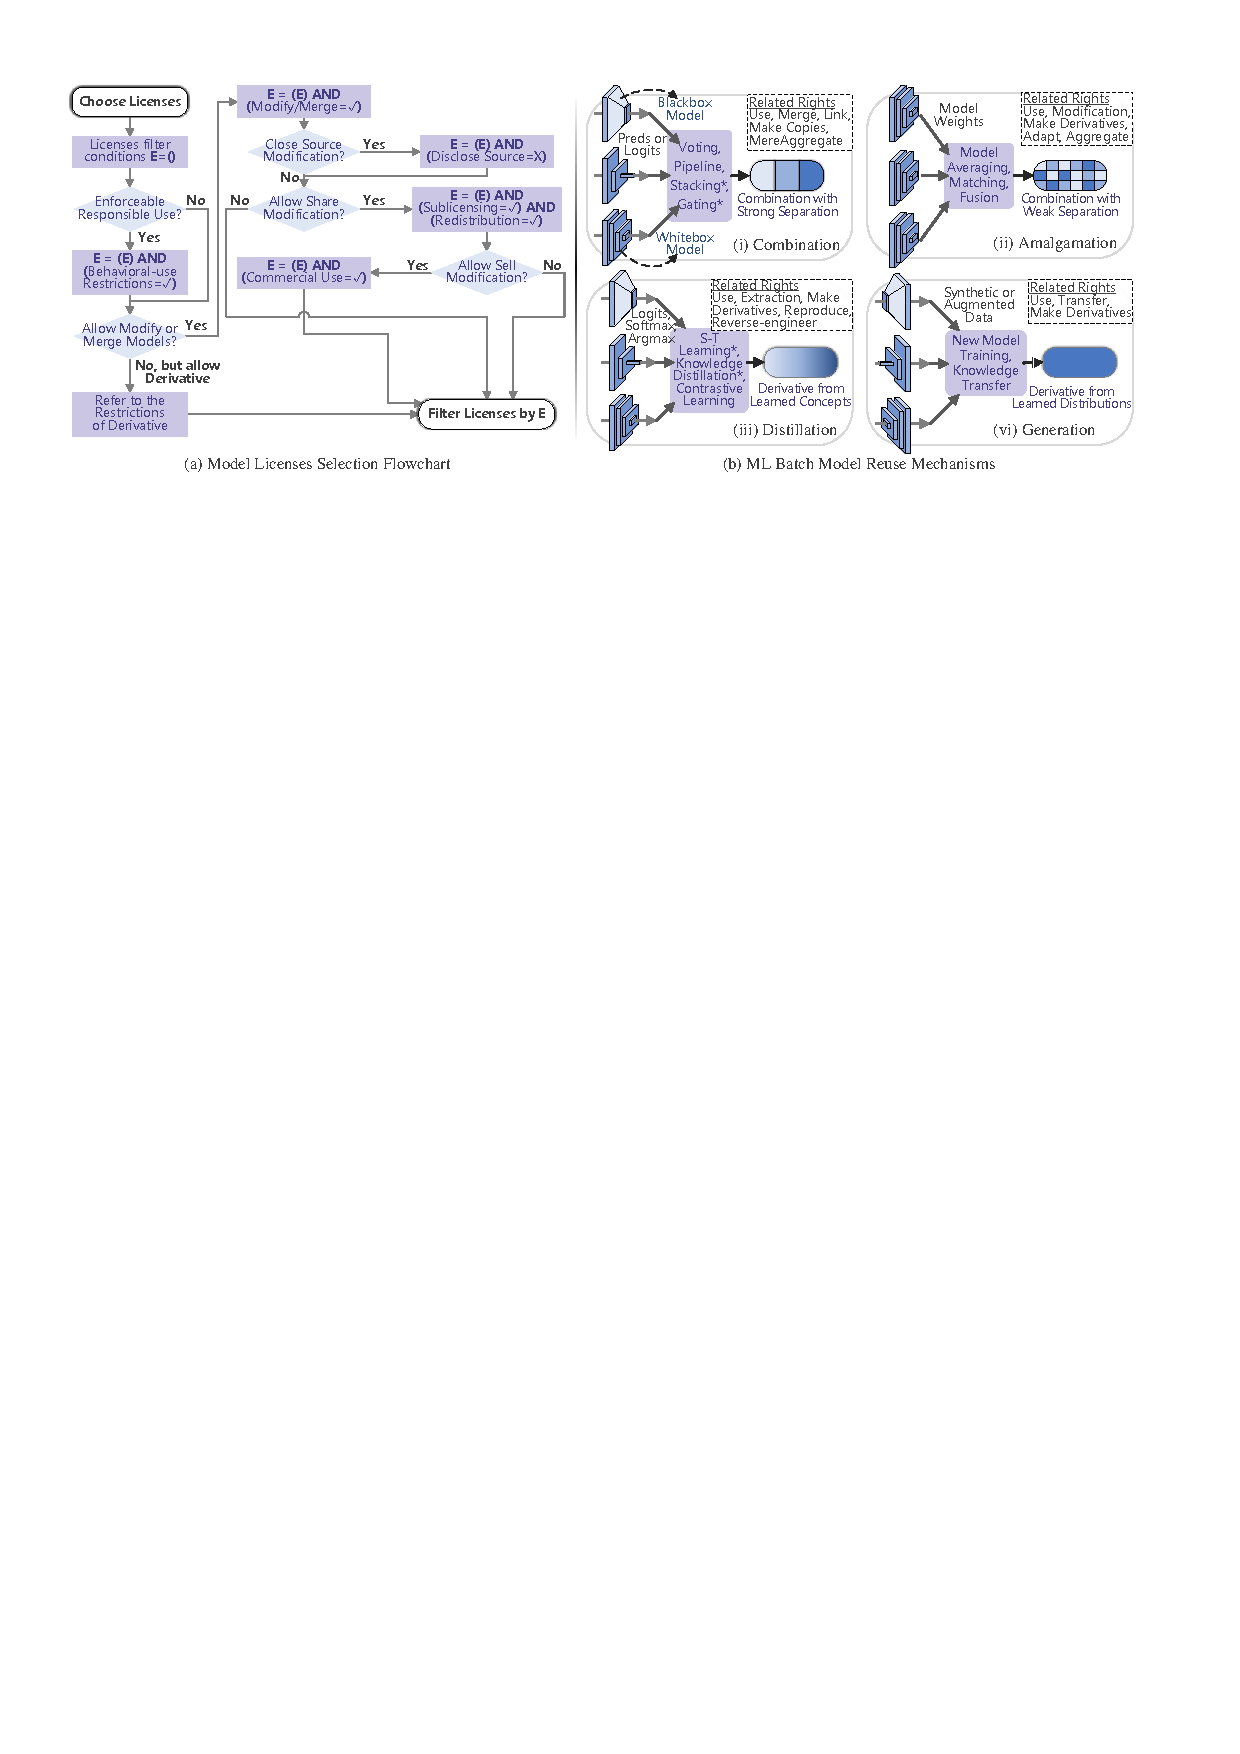
\includegraphics[width=\linewidth]{fig/flowchart.pdf}
    \caption{flowchart}
    \Description{}
    \label{fig:flowchart}
\end{figure}

\textbf{Combination}~\cite{zhou2012ensemble} is a straightforward way to reuse batch of models (aka. base learners), in which multiple models jointly contribute to the output by combination strategies such as averaging, voting, learning~\cite{jacobs1991adaptive, wolpert1992stacked}.
For regression estimates, averaging can improve the generalization by taking the mean of the outputs of all weak learners in a population. Additionally, the outputs of each learner can be weighted by extra parameters~\cite{perrone1995networks}, which can be determined by stacking estimators~\cite{wolpert1992stacked}, Bayes approach~\cite{clarke2003comparing} or backpropagation of gating networks~\cite{jacobs1991adaptive}. 
% Bayesian Model Averaging (BMA) -> Stacking with probabilities
Voting is a workaround for classification tasks and also applicable for stacking and gating.
Both stacking and gating rely on an additional holdout or validation dataset for calculating extra parameters, marked as * in Fig.~\ref{fig:flowchart}(b). 
The difference is that gating can adapt the weights of each model's estimation based on the inputs, providing better generalizability performance of the combined model.

There are many advantages of combination mechanisms from the perspective of FL.
First, the input spaces of base models can be unaligned, which is ideal for the scenario of vertical FL~\cite{wu2022practical} where each client may have inconsistent features in their data.
Secondly, especially for query-based FL, it can simultaneously support multiple types and heterogeneous models, which means that it does not rely on any prior assumptions of the models, such as whether they are DNNs or decision trees, released with weights (whitebox) or binary forms (blackbox).
Thirdly, the tasks of models can be different if we pipeline the base models end-to-end, which is usually overlooked as a combination mechanism of models. 
Pipelining can fully leverage the transferability of models to solve previously unexplored ML problems.
% 举例说明 pipeline
For instance, Gao \textit{et al.}~\cite{gao2022precise} proposed a zero-shot dense retrieval system named HyDE by pipelining a natural language generation (NLG) model~\cite{ouyang2022training} and a natural language understanding (NLU) model~\cite{izacard2021towards}.
The generated content, which may lack factual grounding, from the NLG model is used as query embeddings to facilitate real document retrieval by the NLU model.
Through query-based FL, we can query a vicarious NLG model for a novel scenario, such as ProGen~\cite{madani2023large} for protein sequences generation, and quickly adapt this system to proteomics.
Not limited to that, we can query a batch of NLG models by a well-chosen filter condition and then combine models through averaging or gating to significantly expand the exploration space for knowledge discovery.
Lastly, the combinated models have strong separation from each other, meaning that we can add or remove a batch of models without significant changes to the remaining ones.
Furthermore, combination mechanisms do not rely on the transparency of models and support blackbox sharing. 
Thus, the base model can establish loose connections with other models only through run scripts, providing revocability of such combination and circumvention of the restrictions of licenses.

On the other hand, instead of being treated as a challenge for FL~\cite{ma2022state}, the statistical heterogeneity and model heterogeneity nature of these crowdsourced models can actually enrich population diversity, which is crucial for creating a good ensemble~\cite{maclin1995combining, opitz1995generating}.

\textbf{Amalgamation} involves combining models through model parameters granularity operations, such as median~\cite{blanchard2017machine, pillutla2022robust} and coordinate-wise averaging with consideration of heterogeneity~\cite{mcmahan2017communication, li2018federated}, security~\cite{sun2019can}, scalability~\cite{reisizadeh2020fedpaq}, matching~\cite{wang2020federated, yu2021fed2}, specificality~\cite{gudur2020resource}, generalizability~\cite{qu2022generalized}, resulting in a combination with weak separation.
This reusing approach is widely used in FL works and is often referred to as "aggregation" procedures for local models.
Here, we avoid using the term "aggregation" to distinguish it from "combination". The latter is often used interchangeably with "combination" in software licenses (e.g. Artistic, GPL).

FedAvg~\cite{mcmahan2017communication} is the most popular model averaging method in FL with many follow-up works. 
For instance, Sun \textit{et al.}~\cite{sun2019can} proposed applying norm thresholding of local model updates to defend against backdoor attacks.
Similarly, Blanchard \textit{et al.}~\cite{blanchard2017machine} proposed using more robust median-based amalgamation strategies for resilience against Byzantine behavior.
Consider the ordering of parameters, Wang \textit{et al.}~\cite{wang2020federated} match and average the neural parameters layer-wise across local models, based on their similarities.
However, these methods require multiple rounds of communication to converge, which is not applicable in a query-based FL setting.

Another group of studies leverages Bayesian nonparametrics to learn the shared global latent structures among local models~\cite{yurochkin2019bayesian, yurochkin2019statistical, lam2021model}. 
These methods, known as Model Fusion, can identify distributions of neural components across local models and only fuse the components with the same distribution, which can be explained as a model compression between FedAvg (coordinate-wise averaging) and combination (w/o averaging).
However, the model fusion strategies rely on multiple communication rounds to boost the fusion efficiency, and the model performance of one-shot fusion is even worse than that of Ensemble.

It is worth noting that our taxonomy is based on the form of the resulting model, which may not be entirely consistent with the terminology used in the technical perspective.
For example, Bayes Model Averaging (BMA)~\cite{clarke2003comparing} estimates posterior probabilities of each model given the observed data, which results in a separable weighted model. 
Therefore, it should be classified as Combination instead of Amalgamation like FedAvg.
This novel taxonomy method is useful for analyzing compatibility with licenses. 
For instance, coordinate-wise operations and fusion of model parameters generate fine-grained combinations of models that are almost irreversible, which corresponds to clauses such as adapt, modify, dynamic link, etc., in software licenses.

\textbf{Distillation} was initially proposed by Hinton \textit{et al.}~\cite{hinton2015distilling} to transfer knowledge from a batch of independently trained neural network models (Specialists) to create a new Generalist model.
Their motivation was to explore the parallelization of training of specialists and improve the efficiency of distributed NNs modeling\cite{dean2012large}.
Each specialist only learns fine-grained distinctions of a subset of classes, which is very similar to the non-IID setting in FL~\cite{li2021federated}.
Therefore, it is natural to extend the knowledge distillation to FL filed~\cite{jiang2020federated, li2020practical, li2019fedmd, wu2022communication, chen2020fedbe, lin2020ensemble, gong2021ensemble, sun2020federated}.

Data-Free Knowledge Distillation(DFKD)~\cite{lopes2017data}


% KD 是用于加速网络训练,属于分布式机器学习范畴

% KD 的优点:不需要相同的模型结构,缺点:依赖数据, extracted soft labels

\textbf{Generation}

\begin{table}[]
  \centering
  \footnotesize
  \caption{FL model reuse; \textcolor{purple}{Server} \textcolor{blue}{Client} Knowledge Distillation (KD) Challenges: \textbf{E}fficiency \textbf{H}eterogeneity \textbf{P}rivacy}
  \label{tab:flreuse}
  \begin{tabular}{|p{1.9cm}|p{1.55cm}|p{1.5cm}|p{4.0cm}|p{2cm}|p{1.3cm}|p{0.5cm}|}
    \hline
    \multicolumn{1}{|c|}{FL Studies} & \multicolumn{1}{c|}{\textbf{C}ombination} & \multicolumn{1}{c|}{\textbf{A}malgamation} & \multicolumn{1}{c|}{\textbf{D}istillation} & \multicolumn{1}{c|}{\textbf{G}eneration} & \multicolumn{1}{c|}{Process}& \multicolumn{1}{c|}{Goals} \\ \hline
    FedAvg~\cite{mcmahan2017communication} & &  \textcolor{purple}{Model Avg}  &  &  & [\textcolor{purple}{A}]*N & EH   \\ \hline

    FedAD~\cite{gong2021ensemble} & & & \textcolor{purple}{KD} \textcolor{blue}{\textbf{Attention, Logits}}  & & [\textcolor{purple}{D}]*1 & HP \\ \hline %CC

    FedKD\textsubscript{1}~\cite{gong2022preserving}& & & \textcolor{purple}{KD} \textcolor{blue}{\textbf{Weighted Logits}} & &[\textcolor{purple}{D}]*1 & EHP \\ \hline %CC

    FedMD~\cite{li2019fedmd} &&&\textcolor{blue}{KD \textbf{Logits Avg}} &&[\textcolor{blue}{D}]*N & H \\ \hline %CC

    FedMD-NFDP\newline\cite{sun2020federated}& & & \textcolor{blue}{KD \textbf{Logits/Softmax/Argmax Avg}} & &[\textcolor{blue}{D}]*N & HP \\ \hline %CC

    RHFL~\cite{fang2022robust}& & & \textcolor{blue}{KD \textbf{Weighted Logits}} & &[\textcolor{blue}{D}]*N & EH \\ \hline %CC

    One-Shot FL~\cite{guha2018one} & \textcolor{purple}{Output Avg} & & \textcolor{purple}{KD} \textcolor{blue}{\textbf{Softmax}} & & [\textcolor{purple}{CD}]*1 & EP \\ \hline %CC

    FedDF~\cite{lin2020ensemble} &  & \textcolor{purple}{Model Avg} & \textcolor{purple}{KD}  \textcolor{blue}{\textbf{Logits Avg}} & & [\textcolor{purple}{AD}]*N & HP \\ \hline %CC

    PerAda~\cite{xie2023perada} &  & \textcolor{purple}{Adapter Avg} & \textcolor{purple}{KD} \textcolor{blue}{\textbf{Logits Avg}} & & [\textcolor{purple}{AD}]*N & EHP \\ \hline

    FedDistill~\cite{jiang2020federated}& & \textcolor{purple}{Model Avg} & \textcolor{blue}{KD \textit{Softmax}}& &[\textcolor{blue}{D}\textcolor{purple}{A}]*N & H \\ \hline %CC

    FedFusion~\cite{yao2019towards} & & \textcolor{purple}{Model Avg} & \textcolor{blue}{KD} \textcolor{purple}{\textbf{Hidden}} & & [\textcolor{blue}{D}\textcolor{purple}{A}]*N & E \\ \hline %CC

    FedMLB~\cite{kim2022multi} & & \textcolor{purple}{Model Avg} &\textcolor{blue}{KD} \textcolor{purple}{\textit{Softmax, Scaled Softmax}} & & [\textcolor{blue}{D}\textcolor{purple}{A}]*N & EH \\ \hline %CC

    FedAlign~\cite{mendieta2022local}& &\textcolor{purple}{Model Avg}&\textcolor{blue}{KD}  \textcolor{purple}{\textit{Lipschitz Constants}}~\cite{shang2021lipschitz}& & [\textcolor{blue}{D}\textcolor{purple}{A}]*N & EH \\ \hline %CC

    FedNTD~\cite{lee2022preservation} & & \textcolor{purple}{Model Avg} & \textcolor{blue}{KD} \textcolor{purple}{\textit{Not-True Classes Softmax}} & & [\textcolor{blue}{D}\textcolor{purple}{A}]*N & H \\ \hline %CC

    FedKC~\cite{wang2022fedkc} & & \textcolor{purple}{Model Avg} & \textcolor{blue}{KD} \textcolor{blue}{\textit{Clustered Hidden Avg}} & & [\textcolor{blue}{D}\textcolor{purple}{A}]*N & HP \\ \hline %CC

    MOON~\cite{li2021model} & & \textcolor{purple}{Model Avg} & \textcolor{blue}{Contrastive Learning} \newline \textcolor{purple}{\textit{Hidden}}, \textcolor{blue}{\textit{Hidden}} &&[\textcolor{blue}{D}\textcolor{purple}{A}]*N & EH \\ \hline %CC

    FedCAD~\cite{he2022class} & & \textcolor{purple}{Model Avg} & \textcolor{blue}{KD} \textcolor{purple}{\textbf{Class-Wise Softmax}} &&[\textcolor{blue}{D}\textcolor{purple}{A}]*N & H \\ \hline %CC

    FCCL~\cite{huang2022learn} & & & \textcolor{purple}{Contrastive Learning} \textcolor{blue}{\textbf{Logits Avg}} \textcolor{blue}{Continual Learning} \textcolor{blue}{\textit{Logits}} & & [\textcolor{purple}{D}\textcolor{blue}{D}]*N & H \\ \hline %CC
    
    GFL~\cite{cheng2023gfl} & & \textcolor{purple}{Model Avg} & & \textcolor{blue}{Synthetic Data} & \textcolor{blue}{G}[\textcolor{purple}{A}]*N & HP \\ \hline

    FedSage+~\cite{zhang2021subgraph} & & \textcolor{purple}{Gradient Avg}\newline\textcolor{purple}{Model Avg} & &\textcolor{blue}{Synthetic Node} & [\textcolor{blue}{G}\textcolor{purple}{A}]*N \newline [\textcolor{purple}{A}]*N & H \\ \hline
    
    Fed-ZDAC~\cite{hao2021towards} & & \textcolor{purple}{Model Avg} & & \textcolor{blue}{Synthetic Data of}\newline \textcolor{blue}{Global Model}  & [\textcolor{blue}{G}\textcolor{purple}{A}]*N & HP \\ \hline
    Fed-ZDAS~\cite{hao2021towards} & & \textcolor{purple}{Model Avg} & & \textcolor{purple}{Synthetic Data of} \newline \textcolor{purple}{Local Models} & [\textcolor{purple}{GA}]*N & HP \\ \hline

    DENSE~\cite{zhang2022dense} & \textcolor{purple}{Collection} & & \textcolor{purple}{KD} \textcolor{blue}{\textbf{Logits}} & \textcolor{purple}{Synthetic Data} & [\textcolor{purple}{GCD}]*N & HP \\ \hline %CC

    FedBE~\cite{chen2020fedbe} & & \textcolor{purple}{Model Avg} & \textcolor{purple}{KD} \textcolor{blue}{\textbf{Softmax Avg}} & \textcolor{purple}{Synthetic Model}& [\textcolor{purple}{AGD}]*1 & H \\ \hline %CC

    FedAUX~\cite{sattler2021fedaux}& & \textcolor{purple}{Model Avg} & \textcolor{blue}{Contrastive Learning} \textcolor{purple}{\textbf{Hidden}} \newline \textcolor{purple}{KD} \textcolor{blue}{\textbf{Weighted Logits}} & & \textcolor{blue}{D}[\textcolor{purple}{AD}]*N \newline \textcolor{blue}{D}[\textcolor{purple}{AD}]*1 & HP \\ \hline %CC
    
    FedKD\textsubscript{2}~\cite{wu2022communication} & & \textcolor{purple}{Gradient Avg} & \textcolor{blue}{KD} \textcolor{purple}{\textit{Hidden, Attention, Logits}} \newline \textcolor{blue}{KD} \textcolor{blue}{\textit{Hidden, Attention, Logits}} & & [\textcolor{blue}{D}\textcolor{purple}{A}\textcolor{blue}{D}]*N & EH \\ \hline %CC

    FedKT~\cite{li2020practical} & \textcolor{blue}{Voting} \textcolor{purple}{Voting} & & \textcolor{blue}{KD} \textcolor{blue}{\textbf{Argmax}} \textcolor{purple}{KD} \textcolor{blue}{\textbf{Argmax}} & & [\textcolor{blue}{CD}\textcolor{purple}{CD}]*1 & HP \\ \hline %CC

    FedMatch~\cite{jeong2020federated} & \textcolor{blue}{Voting} & \textcolor{purple}{Model Avg} & \textcolor{blue}{KD} \textcolor{blue}{\textbf{Argmax}} & & [\textcolor{blue}{CD}\textcolor{purple}{AA}]*N \newline [\textcolor{blue}{CD}\textcolor{purple}{A}]*N & EH \\ \hline %CC

    FedGen~\cite{zhu2021data} & & \textcolor{purple}{Model Avg} &\textcolor{purple}{KD} \textcolor{blue}{\textbf{Softmax}} \textcolor{purple}{KD} \textcolor{blue}{\textbf{Logits Avg}} & \textcolor{purple}{Augmented Data} & \textcolor{purple}{D}[\textcolor{blue}{G}\textcolor{purple}{AD}]*N & EHP \\ \hline %CC

    &                       &                       &                       &                       &         &              \\ \hline
    &                       &                       &                       &                       &         &              \\ \hline
    &                       &                       &                       &                       &         &              \\ \hline
  \end{tabular}
\end{table}


\begin{table}[]
  \centering
  \footnotesize
  \caption{model reuse}
  \label{tab:reuse}
  \begin{tabular}{|p{2.2cm}|p{3.55cm}|p{2.8cm}|p{2.8cm}|p{2.7cm}|}
    \hline
    & Combinated Work \newline with Strong Separation & Combinated Work \newline with Weak Separation & Derivative Work \newline from Concepts & Derivative Work \newline from Distributions \\ \hline
    Apache-2.0 & Separable -> Independent Work & Modify -> Derivative & \ding{55} & \ding{55} \\ \hline
    MIT & \ding{55} & \ding{55} & \ding{55} & \ding{55} \\ \hline
    AFL-3.0 & \ding{55} & Modify -> Derivative & \ding{55} & \ding{55} \\ \hline
    GPL-3.0 & Blackbox: Aggregate -> \newline Independent Work \newline Other: Link -> Modified Version  & Modify -> Covered Work & Output no consititutes a covered work -> \newline Independent Work & Output no consititutes a covered work -> \newline Independent Work  \\ \hline
    Artistic-2.0 & Blackbox: MereAggregation ->\newline Independent Work \newline Other: Link -> Modified Version & Aggregate -> \newline Modified Version & \ding{55} & \ding{55} \\ \hline
    BSD-3-Clause & Blackbox: Rredsitribution in \newline binary forms -> \ding{55} \newline Other: Redistribution of source code -> \ding{55} & \ding{55} & \ding{55} & \ding{55} \\ \hline
    WTFPL-2.0 & \ding{55} & \ding{55} & \ding{55} & \ding{55} \\ \hline
    OpenRAIL Licenses & Transfer of patterns of \newline output -> Derivative & Transfer of patterns of weights -> Derivative & Transfer of patterns of activations -> Derivative & Transfer of patterns of output -> Derivative \\ \hline
    Creative Commons \newline Licenses & Reproduce -> Adapted Material & Adapt -> \newline Adapated Material & \ding{55} & \ding{55} \\ \hline
    CC0-1.0 & Reproduce -> \newline Independent Work & Adapt -> \newline Independent Work & \ding{55} & \ding{55} \\ \hline
  \end{tabular}
\end{table}

\begin{comment}
Model type?

Model heterogeneity?

Black box, White box, Mix?

With val?

Horizontal or Vertical?

Query syntax: Table.~\ref{table:repository}, data description, workflow metadata/history of ML pipeline (Scientific workflow management), model performance and profile (task-specific), software dependency,
model use mode
\end{comment}

CreativeML Open RAIL-M:
we added use-based restrictions not permitting the use of the Model in very specific scenarios, in order for the licensor to be able to enforce the license in case potential misuses of the Model may occur.

\subsection{How to Protect Models}